\section{Figures, tables, and display math}
\label{sec:results}

\subsection{Figures}
Figure~\ref{fig:diagram} is the PNG at \texttt{figures/diagram.png}, included
with the \texttt{graphicx} package:

\begin{verbatim}
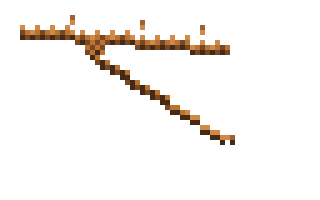
\includegraphics[width=0.62\textwidth]{figures/diagram.png}
\end{verbatim}

\begin{figure}[ht]
  \centering
  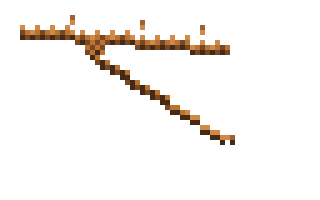
\includegraphics[width=0.62\textwidth]{figures/diagram.png}
  \caption{A small pixel figure shipped with this starter project.}
  \label{fig:diagram}
\end{figure}

Put assets under \texttt{figures/} (or any folder you prefer) and keep the path
in \texttt{\textbackslash includegraphics} in sync with the tree.

\subsection{Tables}
Tables are ordinary \texttt{tabular} environments. The rules below come from
\texttt{booktabs} (\texttt{\textbackslash toprule}, \texttt{\textbackslash midrule},
\texttt{\textbackslash bottomrule}):

\begin{table}[ht]
  \centering
  \begin{tabular}{lrr}
    \toprule
    Method & Error & Time (s) \\
    \midrule
    Baseline & 0.041 & 1.2 \\
    Improved & 0.018 & 1.5 \\
    \bottomrule
  \end{tabular}
  \caption{A compact comparison table using \texttt{booktabs}.}
  \label{tab:compare}
\end{table}

Refer to the table with \texttt{\textbackslash ref\{tab:compare\}} $\to$
Table~\ref{tab:compare}.

\subsection{Aligned math}
Multi-line displays use \texttt{align} from \texttt{amsmath}. The
\verb|&| character marks the alignment point and \verb|\\|
breaks the line:

\begin{align}
  \norm{Ax - b}_2^2
    &= (Ax - b)^\top (Ax - b) \\
    &= x^\top A^\top A x - 2 b^\top A x + b^\top b.
\end{align}

\subsection{Lists and footnotes}
\begin{itemize}
  \item Upload a folder to mirror a local project layout.
  \item Drag files between folders in the file tree.
  \item Keep experimenting: change numbers in Table~\ref{tab:compare} and
        recompile to see the PDF update.
\end{itemize}

A short footnote can hold an aside.\footnote{Footnotes are written with
\texttt{\textbackslash footnote\{...\}} right where the mark should appear.}
Equation~\eqref{eq:euler} was introduced in Section~\ref{sec:intro}.
